\documentclass[aspectratio=169,10pt]{beamer}

%% CrossCorr -- HamSCI Science Telecon, 5 November 2026
%% Dark theme, palette from aep/CC_Data.js (PALETTE).
%% Every number is verified against paper/main.tex (v1.3.1) by
%% tmp_fix_pres_1_slides.py (Phase 1 anchors).

\usepackage[T1]{fontenc}
\usepackage{graphicx}
\usepackage{booktabs}
\usepackage{amsmath}
\usepackage{helvet}
\renewcommand{\familydefault}{\sfdefault}

\definecolor{ccbg}{HTML}{060911}
\definecolor{cccyan}{HTML}{5CE1DB}
\definecolor{cctext}{HTML}{F1F5FB}
\definecolor{ccdim}{HTML}{828BA0}
\definecolor{ccwarn}{HTML}{FFBF4C}

\usetheme{default}
\mode<presentation>{
  \setbeamercolor{background canvas}{bg=ccbg}
  \setbeamercolor{normal text}{fg=cctext,bg=ccbg}
  \setbeamercolor{alerted text}{fg=cccyan}
  \setbeamercolor{structure}{fg=cccyan}
  \setbeamercolor{frametitle}{fg=cccyan,bg=ccbg}
  \setbeamercolor{title}{fg=cctext}
  \setbeamercolor{subtitle}{fg=ccdim}
  \setbeamercolor{institute}{fg=ccdim}
  \setbeamercolor{date}{fg=ccdim}
  \setbeamercolor{itemize item}{fg=cccyan}
  \setbeamercolor{itemize subitem}{fg=ccdim}
  \setbeamercolor{enumerate item}{fg=cccyan}
  \setbeamercolor{page number in head/foot}{fg=ccdim}
  \setbeamerfont{frametitle}{series=\bfseries,size=\large}
  \setbeamerfont{title}{series=\bfseries,size=\Large}
  \setbeamertemplate{navigation symbols}{}
  \setbeamertemplate{itemize items}[circle]
  \setbeamertemplate{footline}{\hskip1em\usebeamertemplate{page number in head/foot}\hfil}
}

\title{Scale-dependent WSPR response to geomagnetic storms}
\subtitle{Frequency dependence and exploratory period-to-period scaling of
absolute loss}
\author{Alexey Petrov \and Makar Petrov}
\institute{Independent researchers, Russia}
\date{HamSCI Science Telecon --- 5 November 2026}

\begin{document}

%% ------------------------------------------------------------------ 1
\begin{frame}[plain]
  \titlepage
  \vfill
  \begin{center}
    \small\textcolor{ccdim}{M.\ Petrov --- co-author, not presenting
      \quad$\cdot$\quad Version DOI: 10.5281/zenodo.23402384}
  \end{center}
\end{frame}

%% ------------------------------------------------------------------ 2
\begin{frame}{Why WSPR?}
  \begin{itemize}
    \item WSPR (Weak Signal Propagation Reporter): low-rate digital
      mode used by amateur radio operators worldwide
    \item Every received spot is an opportunistic probe of one HF
      propagation path
    \item Public database: who heard whom, when, on which band
    \item Global, continuous, free --- a \alert{distributed
      ionospheric sensor}
    \item Question: does storm activity suppress HF propagation,
      as seen in spot counts?
  \end{itemize}
\end{frame}

%% ------------------------------------------------------------------ 3
\begin{frame}{Data and method}
  \begin{center}
    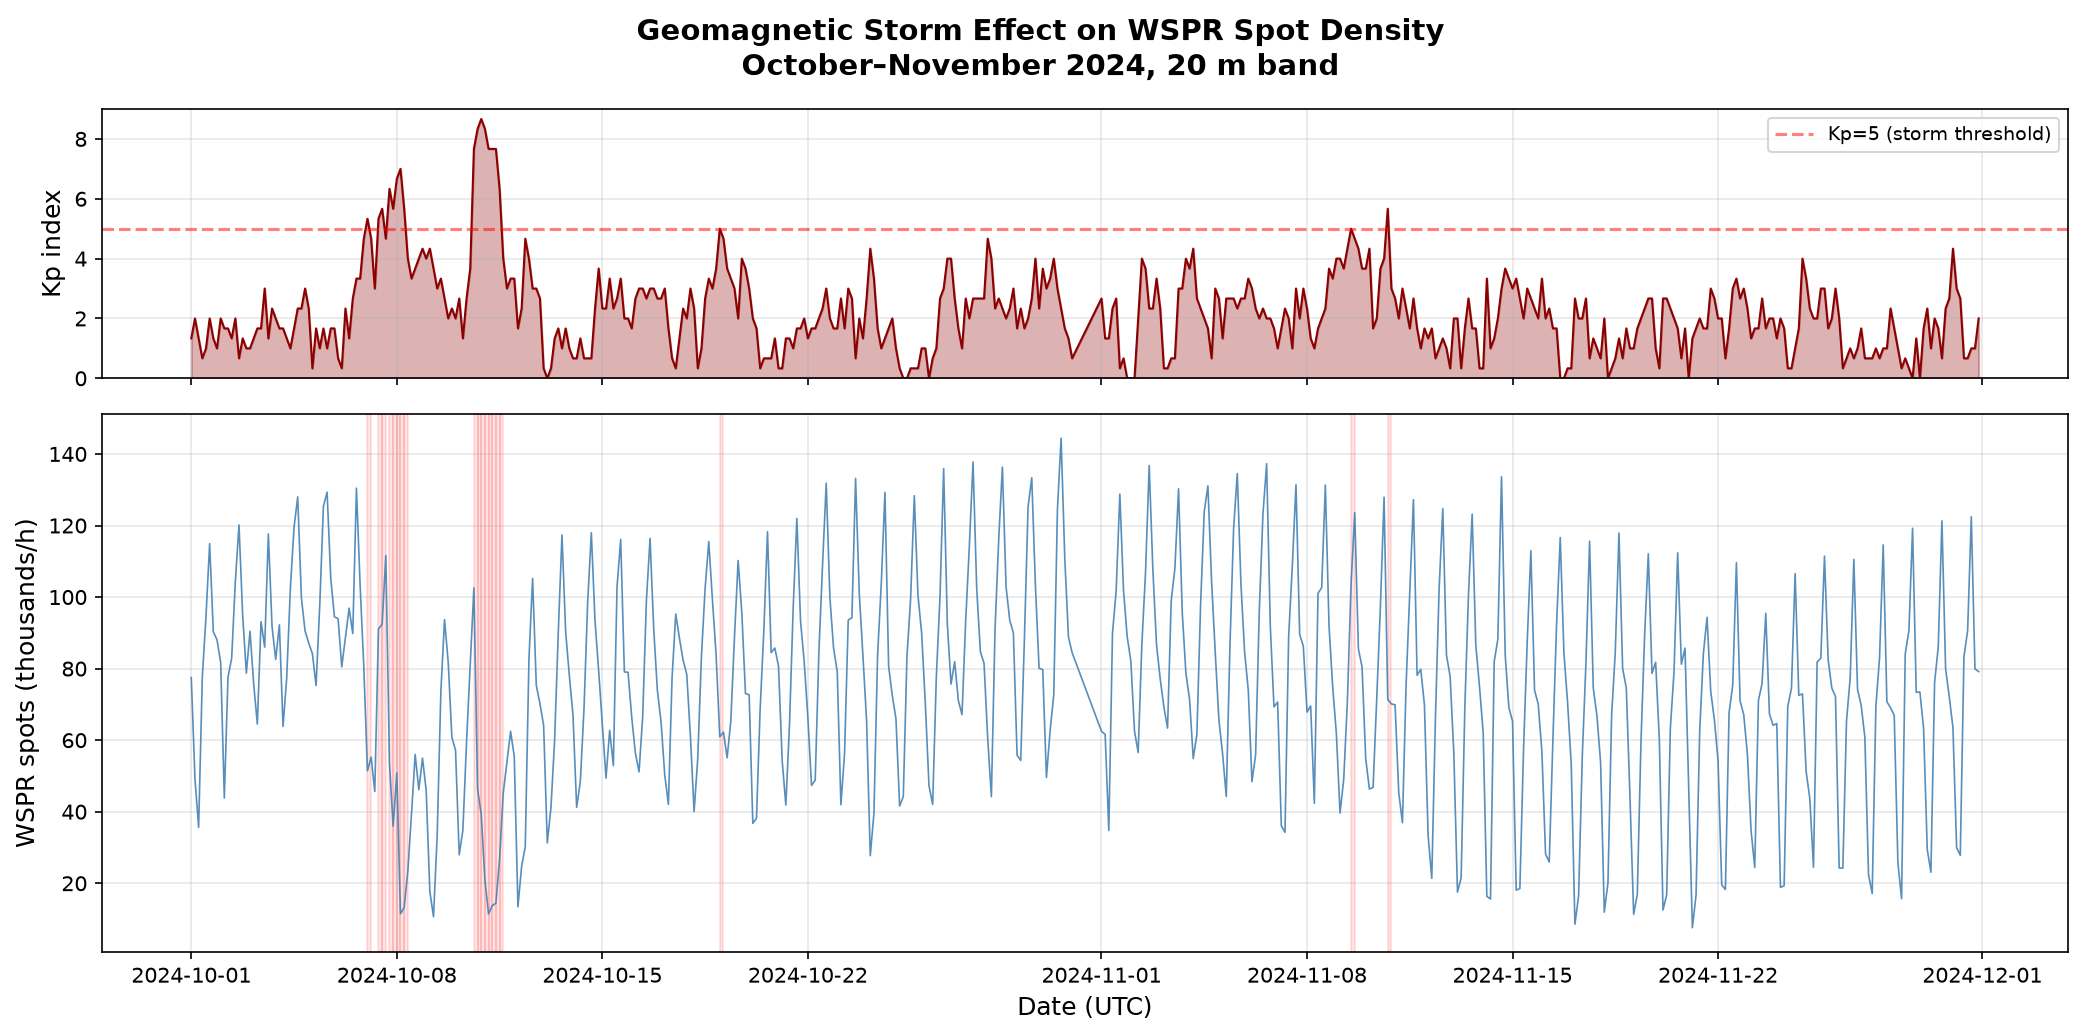
\includegraphics[width=0.70\textwidth,keepaspectratio]{figures/fig1_kp_timeseries.png}
  \end{center}
  \vskip-0.3cm
  \begin{itemize}
    \item \alert{18 months}, Apr 2024 --- Sep 2025; three bands:
      20\,m, 40\,m, 15\,m
    \item 39\,456 WSPR hours across the three bands; hourly counts merged
      3-hourly with the GFZ Potsdam $Kp$ index
    \item Per band: 4\,349 epochs --- \alert{198 storm} ($Kp\ge5$)
      vs 3\,035 quiet ($Kp<3$)
    \item \alert{Block permutation test}: 50\,000 iterations,
      block $=$ 24 epochs $=$ 72\,h; Benjamini--Hochberg FDR
    \item Confirmed independently with $Dst<-50$\,nT (Kyoto, provisional)
  \end{itemize}
\end{frame}

%% ------------------------------------------------------------------ 4
\begin{frame}{Result 1 --- frequency dependence and scale dependence}
  \begin{columns}[T]
    \column{0.44\textwidth}
      \centering
      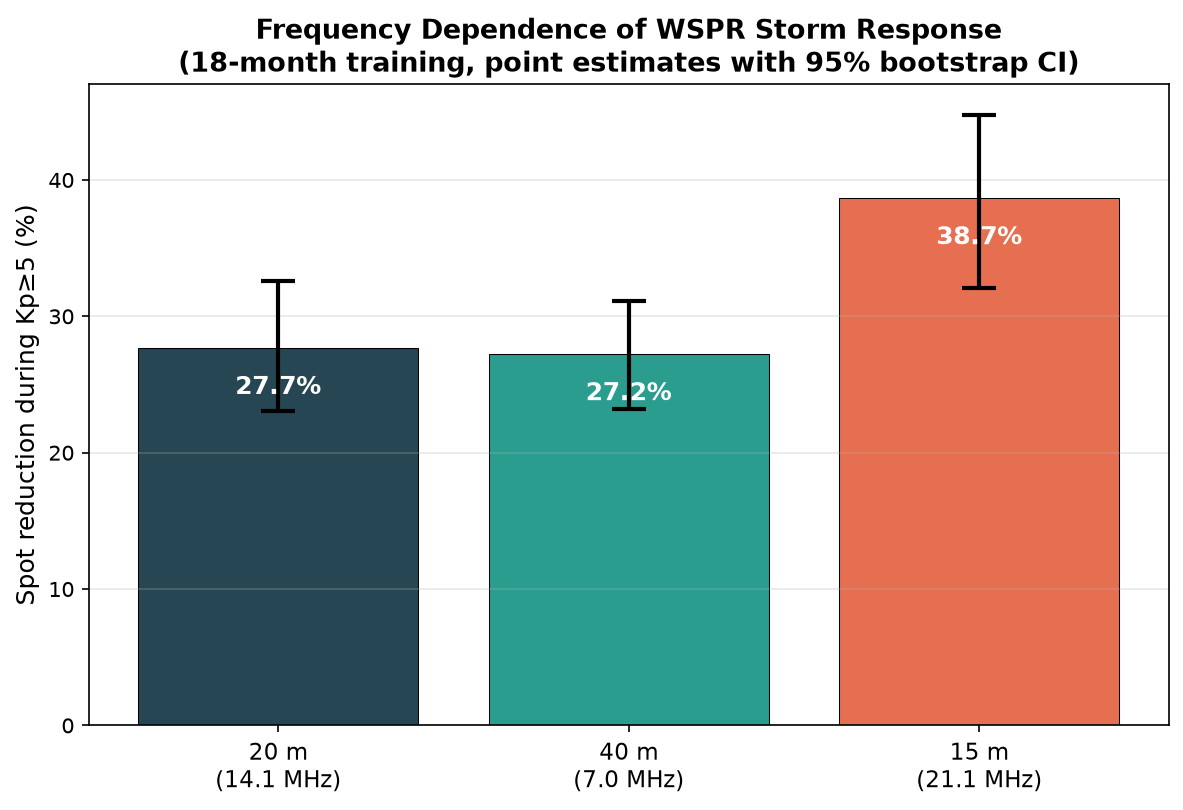
\includegraphics[width=\textwidth,keepaspectratio]{figures/fig3_frequency_dependence_pointest.png}\\
      {\small\textcolor{ccdim}{Spot reduction per band}}
    \column{0.54\textwidth}
      \centering
      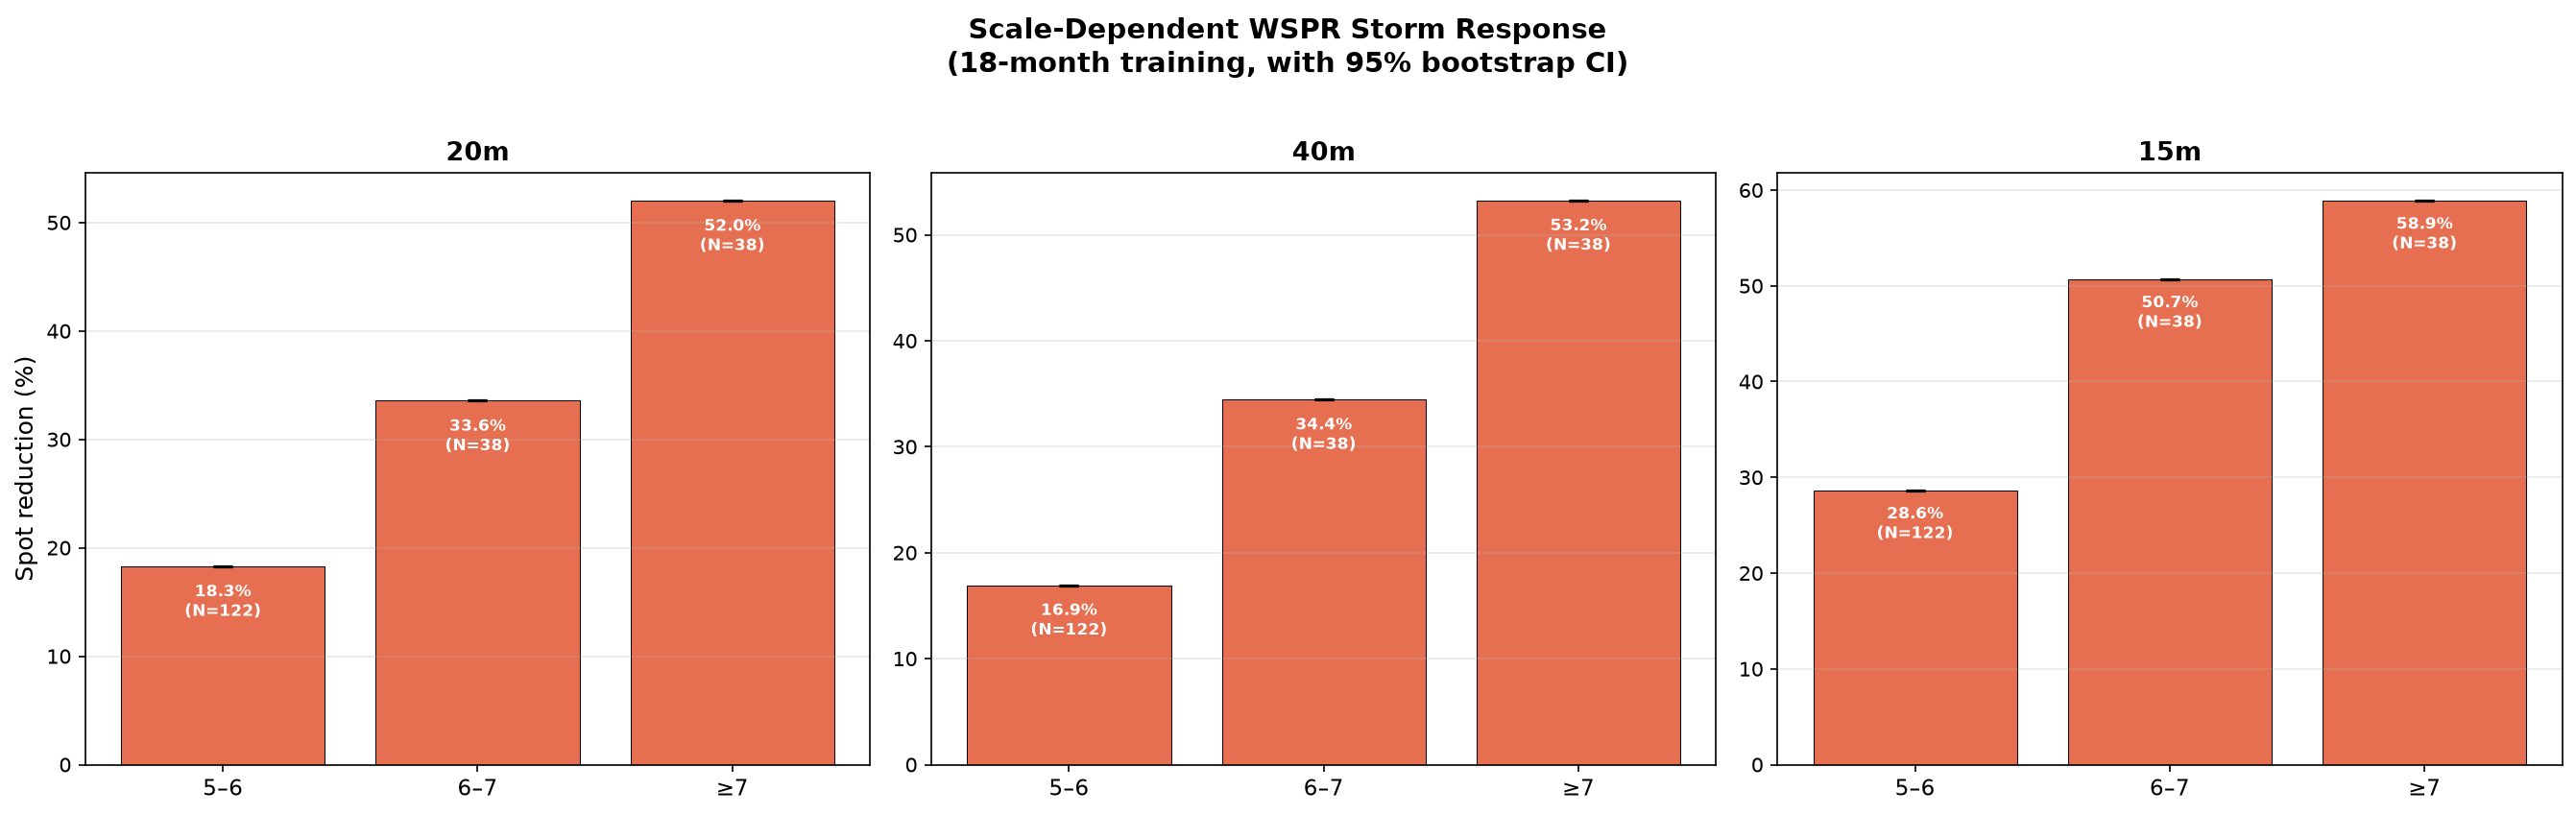
\includegraphics[width=\textwidth,keepaspectratio]{figures/fig2_scale_dependence.png}\\
      {\small\textcolor{ccdim}{Reduction vs storm intensity ($Kp$ bins)}}
  \end{columns}
  \vskip0.1cm
  \begin{itemize}
    \item Raw drops: \alert{20\,m $-27.7\,\%$},
      \alert{40\,m $-27.2\,\%$}, \alert{15\,m $-38.7\,\%$};
      each $p\le2\times10^{-5}$
    \item Gradient: stronger with $Kp$ (see right panel); trend
      significant, highest bin sparse (12 episodes)
    \item Pattern \emph{consistent with} two mechanisms: MUF reduction
      (15\,m) and D-region absorption (20/40\,m)
  \end{itemize}
\end{frame}

%% ------------------------------------------------------------------ 5
\begin{frame}{Result 2 --- UT-window asymmetry}
  \begin{center}
    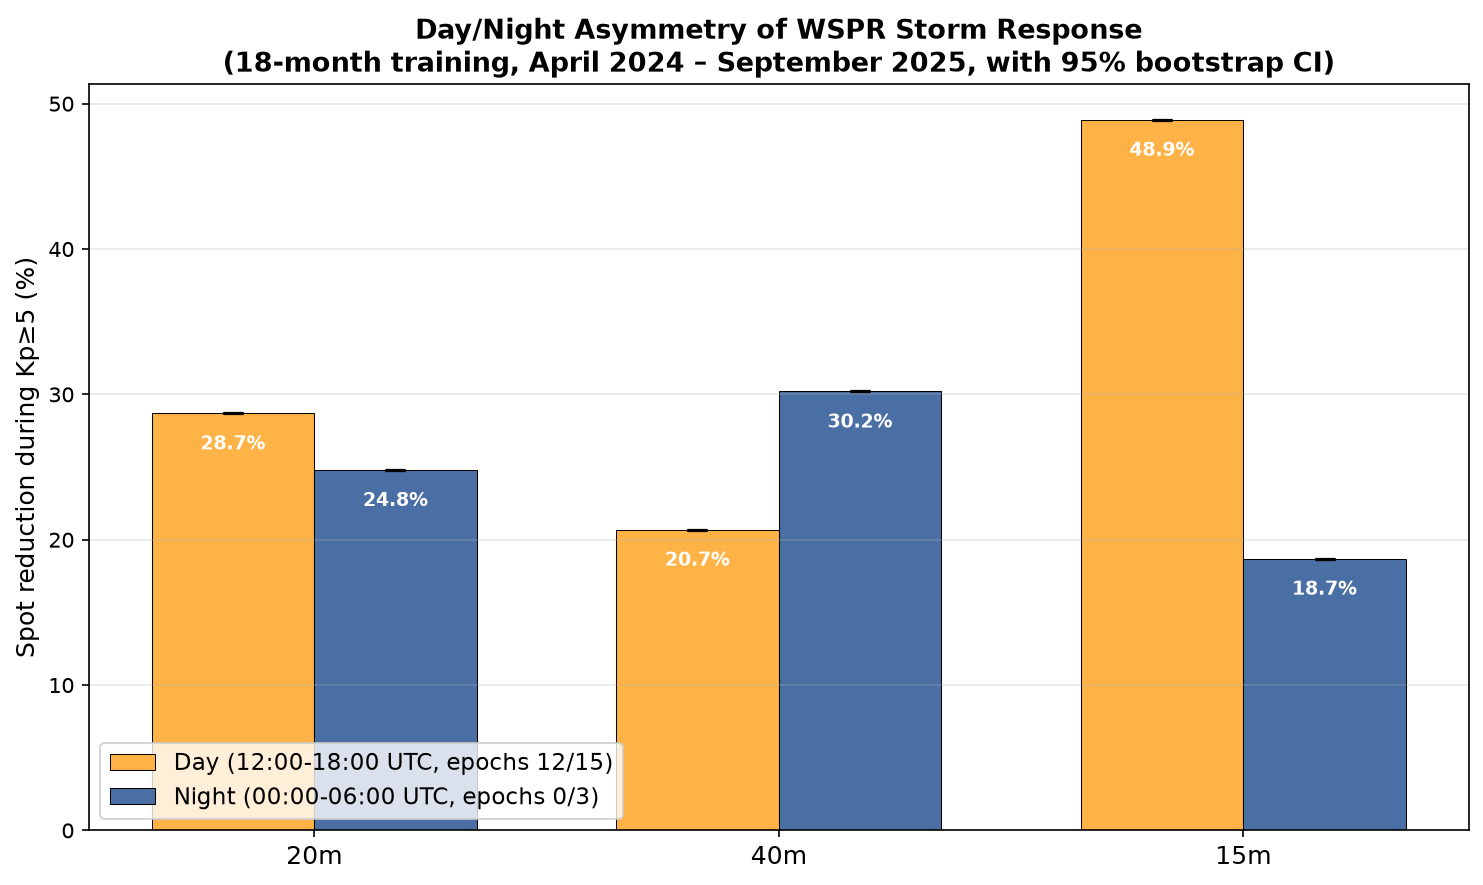
\includegraphics[width=0.58\textwidth,keepaspectratio]{figures/fig4_day_night_asymmetry.png}
  \end{center}
  \vskip-0.15cm
  \begin{itemize}
    \item UT-day (12--18 UTC): 15\,m $-48.9\,\%$ $>$ 20\,m $-28.7\,\%$
      $>$ 40\,m $-20.7\,\%$
    \item UT-night (0--6 UTC): \alert{40\,m $-30.2\,\%$} $>$ 20\,m $-24.8\,\%$
      $>$ 15\,m $-18.7\,\%$
    \item UT-night excess on 40\,m: auroral / polar-cap absorption,
      scaling as $1/f^2$
  \end{itemize}
  \vskip0.1cm
  {\small\textcolor{ccdim}{Training period. The UT-window asymmetry is based
  on training data; the held-out window does not independently resolve
  this (47 storm epochs).}}
\end{frame}

%% ------------------------------------------------------------------ 6
\begin{frame}{Result 3 --- absolute loss on 40\,m: invariance?}
  \begin{center}
    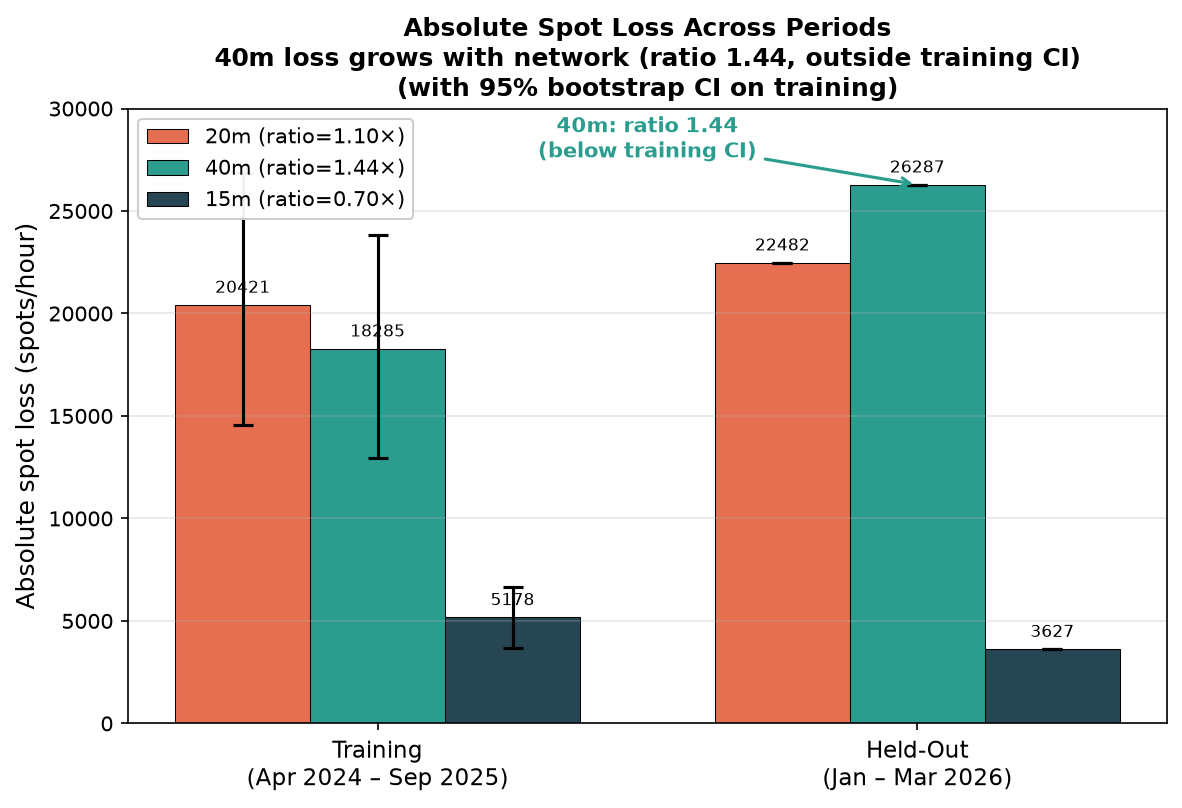
\includegraphics[width=0.48\textwidth,keepaspectratio]{figures/fig5_baseline_invariance.png}
  \end{center}
  \vskip-0.35cm
  \begin{itemize}
    \item Training: $-18\,285$ spots/h, 95\% CI $[-23\,807,\ -12\,930]$
    \item Initial held-out snapshot: $-18\,304$ spots/h
      $\Rightarrow$ ratio $1.00$
    \item Live re-download (15 Oct 2026): $-26\,287$ spots/h,
      CI $[-37\,144,\ -12\,472]$ $\Rightarrow$ \alert{ratio $1.44$}
      (95\% CI $[0.65,\ 2.33]$)
    \item Network grew $+35\,\%$ (40\,m quiet baseline); expected ratio
      $\approx 1.35$ under proportional scaling
    \item Ratio CI also includes $1$: \alert{compatible with proportional
      scaling, but not conclusively established}; percentage drops remain
      the more stable metric
  \end{itemize}
\end{frame}

%% ------------------------------------------------------------------ 7
\begin{frame}{Held-out replication --- Jan--Mar 2026}
  \begin{center}
  \small
  \begin{tabular}{lr}
    \toprule
    Band & Raw reduction \\
    \midrule
    20\,m & $-26.7\,\%$ \\
    40\,m & $-29.0\,\%$ \\
    15\,m & $-22.1\,\%$ \\
    \bottomrule
  \end{tabular}
  \end{center}
  {\small\textcolor{ccdim}{$N_{\mathrm{total}}=720$, $N_{\mathrm{storm}}=47$ per band.}}
  \vskip0.1cm
  \begin{itemize}
    \item Primary effect replicates in direction on \alert{all three bands}
      under the residual permutation test
      ($p\le2\times10^{-4}$; 15\,m raw 95\% CI includes zero)
    \item Scale-dependence at $Kp$ 6--7 agrees within factors $1.01$--$1.12$
      (only 10 storm epochs per band: directional check)
  \end{itemize}
\end{frame}

%% ------------------------------------------------------------------ 8
\begin{frame}{Limitations}
  \begin{itemize}
    \item 18 months in a solar-maximum phase --- not a solar-cycle study
    \item Held-out power: 47 storm epochs; secondary effects
      (UT-window asymmetry) not independently re-tested
    \item 15\,m held-out raw 95\% CI still includes zero
      (residual-based $p$ is significant)
    \item UT windows (12--18 / 0--6 UTC) are not local day/night
      for a global network
    \item Distance bins: strongest loss on 5--10\,000\,km paths;
      no latitude or local-time resolution yet
    \item Spot counts conflate propagation with station activity
      (no active-transmitter normalisation)
    \item F10.7 only monthly; SIDs not separated; 15\,m effect is present
      in all seasons and not driven by summer sporadic-$E$
    \item 198 storm epochs $\approx$ 58 independent episodes
      ($N_{\mathrm{eff}}$); Dst is provisional
    \item Decoded-spot SNR changes by $<0.5$\,dB: the loss is mainly
      marginal paths dropping below the decoding threshold
  \end{itemize}
\end{frame}

%% ------------------------------------------------------------------ 9
\begin{frame}{Conclusions}
  \begin{enumerate}
    \item Storms ($Kp\ge5$) cut WSPR spot density by $27$--$39\,\%$
      raw ($p\le2\times10^{-5}$)
    \item The scale-dependent pattern: $\sim-18\,\%$ at $Kp$ 5--6,
      $\sim-34\,\%$ at $Kp$ 6--7, $\sim-53\,\%$ at $Kp\ge7$;
      trend significant, highest bin sparse
    \item It \alert{replicates in direction} on the held-out Jan--Mar 2026 window
      (all three bands, $p\le2\times10^{-4}$)
    \item Absolute loss is \alert{compatible with network-related scaling}
      (ratio $1.44$, 95\% CI $[0.65, 2.33]$), but not conclusively
      established; percentage drops remain the more stable metric
    \item Frequency/UT pattern is \emph{consistent with} a dual mechanism:
      MUF reduction (15\,m) and D-region absorption (20/40\,m)
  \end{enumerate}
  \vskip0.3cm
  \begin{center}
    WSPR is a viable \alert{distributed ionospheric sensor} for
    storm-driven HF degradation.
  \end{center}
\end{frame}

%% ------------------------------------------------------------------ 10
\begin{frame}[plain]{}
  \vfill
  \begin{center}
    {\Huge\bfseries Questions?}\\[0.7cm]
    {\large\textcolor{ccdim}{Thank you for listening.}}\\[0.9cm]
    {\small
      Paper (v1.3.1): \texttt{10.5281/zenodo.23402384}\\[4pt]
      Concept DOI: \texttt{10.5281/zenodo.23285958}\\[4pt]
      Code: \texttt{github.com/FelixRLEPERS/crosscorr}\\[4pt]
      M.\ Petrov --- co-author, not presenting}
  \end{center}
  \vfill
\end{frame}

\end{document}
